\documentclass[tikz]{standalone}
\usetikzlibrary{
  arrows.meta,                        % for arrow tips
  backgrounds,                        % for background layer
  ext.paths.ortho,                    % for ortho paths
  ext.positioning-plus,               % for 
  ext.node-families.shapes.geometric, % loads ext.node-families and
% shapes.geometric,                   % for ellipse
  calc, positioning}                               % for ($<calculations>$)
\tikzset{
  basic box/.style={
    shape=rectangle, rounded corners, align=center, draw=#1, fill=#1!25},
  header node/.style={
    node family/width=header nodes,
    font=\strut\Large\ttfamily,
    text depth=+.3ex, fill=white, draw},
  header/.style={%
    inner ysep=+1.5em,
    append after command={
      \pgfextra{\let\TikZlastnode\tikzlastnode}
      node [header node] (header-\TikZlastnode) at (\TikZlastnode.north) {#1}
      % the next node contains both \tikzlastnode and its header
      % this is needed so that h-<name> can be used to connect lines
      node [span=(\TikZlastnode)(header-\TikZlastnode)]
           at (fit bounding box) (h-\TikZlastnode) {}
    }
  },
  fat blue line/.style={ultra thick, blue}
}
\begin{document}
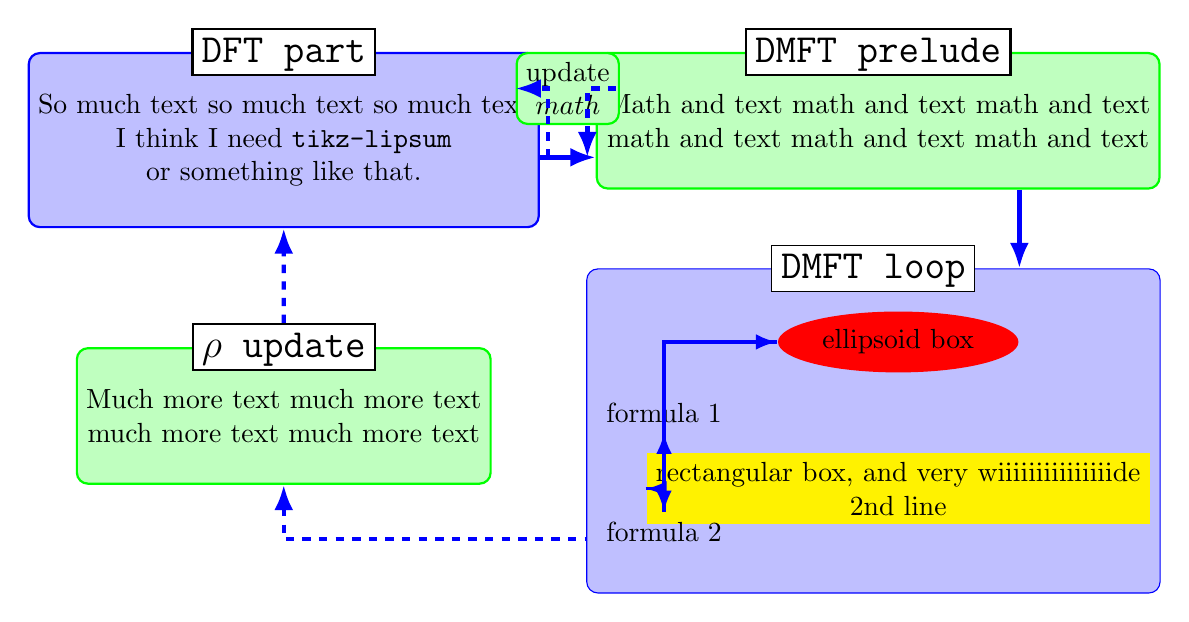
\begin{tikzpicture}[
  node distance=1cm and 1.2cm,
  thick,
  nodes={align=center},
  >={Latex[scale=.9]},
  ortho/install shortcuts]

\path[node family/width=loop]
  node[shape=ellipse, fill=red]       (imp-sol) {ellipsoid box}
  node[fill=yellow, below=of imp-sol] (rec-box) {
    rectangular box, and very wiiiiiiiiiiiiiiide \\ 2nd line};
\node at ($(imp-sol.west|-imp-sol.south)!.5!(rec-box.north west)$) [
  shift=(left:.5*x_node_dist)]  (for-1) {formula 1};
\node [
  below=of for-1] (for-2) {formula 2};

\scoped[on background layer]
  \node[
    basic box=blue, header=DMFT loop,
    fit=(for-1)(for-2)(imp-sol)(rec-box)] (dmft-l) {};

\path[very thick, blue, -|] (rec-box) edge[->] (for-1) edge[<-] (for-2)
                            (imp-sol) edge[->] (for-2) edge[<-] (for-1);

\node[
  basic box=green, header=DMFT prelude,
  east above=of dmft-l] (dmft-p) {
    Math and text math and text math and text \\
    math and text math and text math and text};
\node[
  basic box=green, header=$\rho$ update,
  north left=of dmft-l,  shift=(down:y_node_dist)] (rho) {
    Much more text much more text \\ much more text much more text};
\node[basic box=blue, header=DFT part, anchor=north] at (dmft-p.north-|rho)
  (dft) {So much text so much text so much text \\
            I think I need \texttt{tikz-lipsum} \\ or something like that.};
\node [basic box=green, below=+0pt of (dft.north east)(dmft-p.north west)]
  (upd) {update\\$math$};

\coordinate (dmft-p-sse) at ($(dmft-p.south)!.5!(dmft-p.south east)$)
 coordinate (dmft-l-ssw) at ({$(rho.south)!.5!(dmft-l.south)$}-|dmft-l.south west)
 coordinate (dmft-p-ssw) at ({$(upd.south)!.5!(dmft-p.south)$}-|dmft-p.south west);

\path[fat blue line, ->]
  (rho) edge[<-, dashed, |-] (dmft-l-ssw)
  (dmft-p-ssw) edge[<-, -*] coordinate[pos=.15] (@s)
                            coordinate[pos=.85] (@e) (dft)
  {[every edge/.append style=dashed, |-] (@s) edge[<-] (upd)
                                         (@e) edge     (upd)}
  (h-rho)      edge[dashed] (dft)
  (dmft-p-sse) edge[|*]     (dmft-l);
\end{tikzpicture}
\end{document}
